\setcounter{page}{0}
\chapter{\chapternameintro}

  \the\linewidth

  O período de entrega de dissertações e teses é caótico e no caminho surgem muitas dúvidas: como faço pra depositar? Quais documentos preciso preparar? Onde imprimir a tese? Existem outros prazos que eu deva ficar atento?

  Com o objetivo de ajudar quem estiver nessa etapa, resolvemos criar este documento que, além de servir como um template não oficial para as teses do IAG, também serve como um guia geral.

  \section{Dicas gerais}

    Quando você estiver escrevendo o texto, deve ficar atento aos capítulos que são obrigatórios, seguindo as normas do IAG. Você pode encotrá-las aqui: \url{https://leginf.usp.br/?resolucao=resolucao-copgr-no-7882-de-25-de-novembro-de-2019}. A parte do texto que diz o que é necessário para realizar o depósito está na seção ``XI - PROCEDIMENTOS PARA DEPÓSITO DA DISSERTAÇÃO/TESE''.

    Resumidamente, a dissertação/tese deve conter: Capa, folha de rosto, resumo em português, resumo em inglês, a lista de figuras, ilustrações, tabelas e acrônimos, introdução, metodologia, resultados, conclusões, perspectivas, bibliografia e, opcionalmente, apêndices e anexos.

    Para a tese de doutorado, você também tem a opção de fazer uma coletânea de artigos. Neste caso é necessário ter pelo menos um artigo submetido e/ou publicado e, para poder utilizá-lo na tese, é preciso ter a autorização da(s) editora(s) e dos co-autores. Então você deve incluir um capítulo após a introdução descrevendo a relação entre os artigos e a tese. É possível misturar capítulos ``normais'' e de artigos para construir uma tese coerente.

    O processo de depósito consiste em entregar uma cópia impressa da dissertação/tese na coordenação do programa. Já a manifestação do orientador dizendo que você está apto(a) a defender, o formulário de sugestão da banca, e o comprovante de artigo publicado (no caso do doutorado) devem ser incluídos no depósito eletrônico, realizado na plataforma Janus.

    No Janus, depois de fazer login, você deve ir em ``Aluno regular'' > ``Depósito''. Lá você terá que preencher algumas informações como seu nome (no formato que aparece em citações), o seu ORCID, e anexar os formulários descritos acima, a tese, e o \textbf{protocolo de recebimento de depósito} (Figura \ref{fig:protocolo}), que será feito quando você depositar o exemplar impresso. Fique atento pois você precisará colocar o título, o resumo, e as palavras-chave do seu trabalho em português e inglês, independente de qual é o idioma no qual você escreveu a tese. Além disso, as palavras-chave podem ter no máximo 150 caracteres, e o resumo não pode passar do limite de 5000 caracteres.
    %
    \begin{figure}[h]
      \centering
      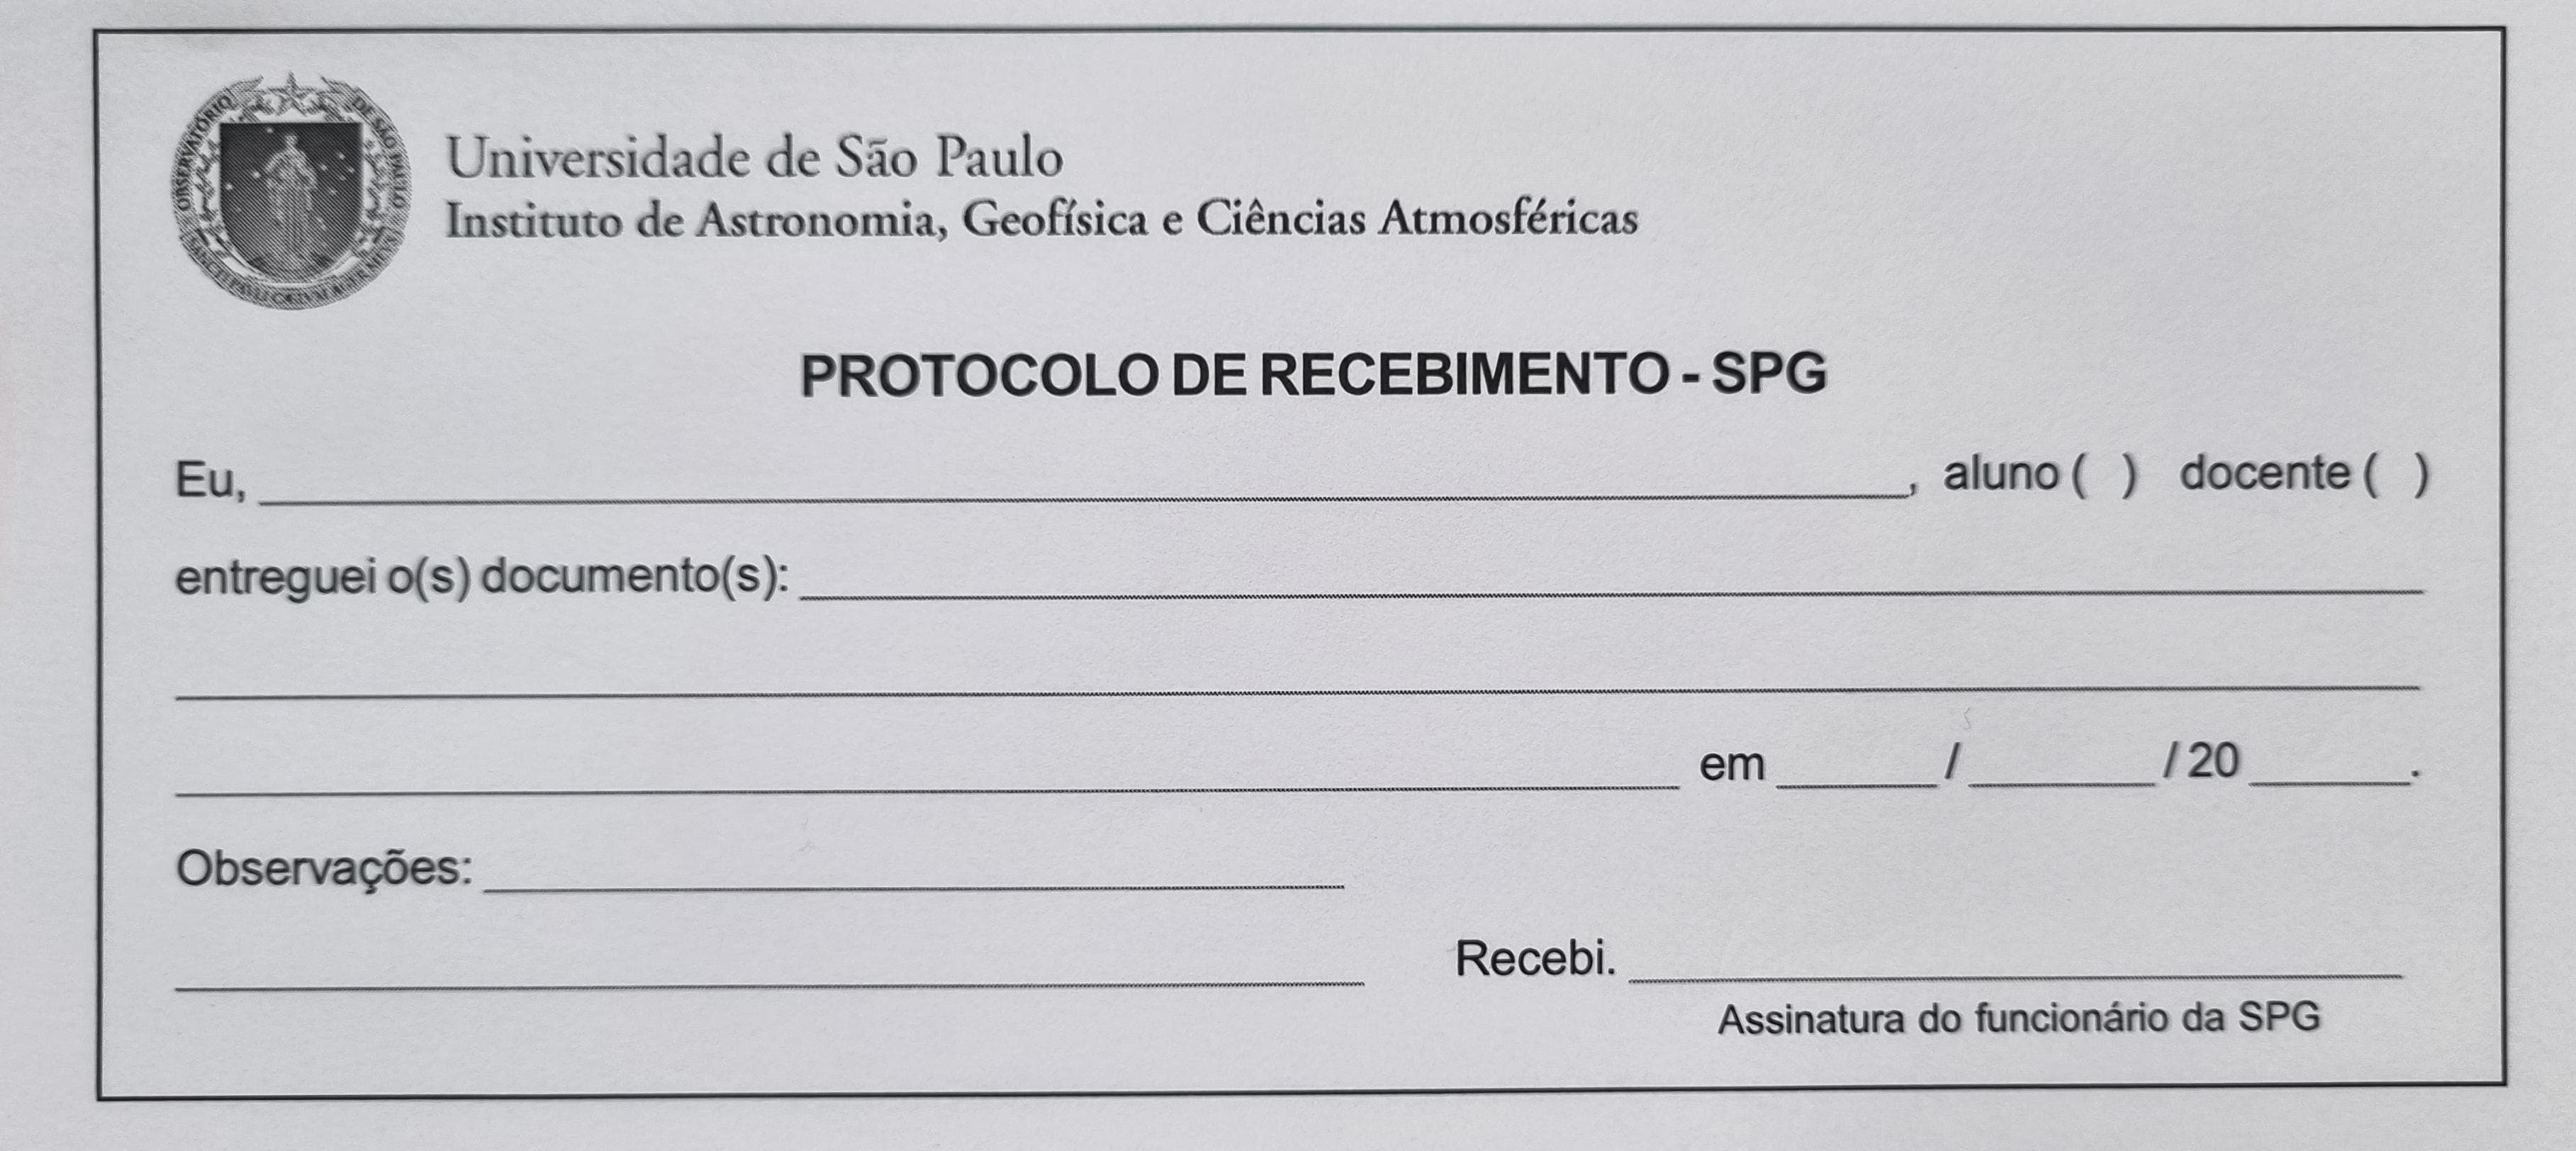
\includegraphics[width=\linewidth]{protocolo_recebimento.jpeg}
      \caption{Foto do protocolo de recebimento de depósito, que você precisa escanear e colocar no Janus.}
      \label{fig:protocolo}
    \end{figure}

    Para imprimir a tese, você pode aproveitar a parceria que o IAG tem com a gráfica do IME. Você só precisa mandar um email para a CCP (\url{ccpastro iag.usp.br}) pedindo autorização. Quando ela for dada, é só encaminhar o email para a Cida (\url{cida.coelho@iag.usp.br}), que fará a solicitação junto à grafica. Quando a impressão estiver pronta, depois de um ou dois dias, ela irá te avisar para você poder fazer a retirada. Note que talvez você tenha que falar com outra pessoa ao invés da Cida quando fizer a solicitação (este texto foi escrito em 2024).

    Tanto o formulário de sugestão da banca quanto a carta de manifestação do orientador estão disponíveis na seção de formulários do site do IAG (\url{https://www.iag.usp.br/pos-graduacao/formularios}), na parte ``8 - Defesa de Dissertações e Teses''. Para a sugestão da banca, a maioria dos examinadores deverá ser de fora do programa e pelo menos um de fora do IAG. Para o mestrado são necessários três titulares e três suplentes, enquanto que no doutorado são 5 titulares e 5 suplentes. Em ambos os casos você precisa colocar o nome do seu orientador(a) e um suplente correspondente. Recomendo você começar a conversar sobre os nomes um mês antes da data que você deseja fazer o depósito, assim você pode enviar emails para os examinadores perguntando se aceitam compor sua banca.

    Depois de entregar os documentos, a CCP irá julgar a sugestão para a banca e, caso aprovada, você terá até 105 dias para realizar a defesa. Caso queira defender em menos de 30 dias, é necessário preencher um termo de responsabilidade (também presente na parte de formulários do site do IAG).

  \section{Características deste template}
    Este template foi criado tendo como base o repositório Web\LaTeX{}, que por sua vez foi criado para substituir o Overleaf. A vantagem neste caso é a integração com o GitHub, permitindo o controle de versões, por exemplo, o uso de Codespaces (que são computadores virtuais, criados através do GitHub) caso você queira, e a possibilidade de usar extensões como Grammarly, LTex e Copilot. Caso você não queira usar um Codespace (pois ele é limitado a 180 horas de uso por mês), você também pode clonar o repositório pra o seu PC e trabalhar normalmente. Isso é possível pois o WebLaTex define um container com toda a informação necessária para você compilar seus documentos.

    \subsection{Web\LaTeX{}}
      O WebLaTex foi criado como uma alternativa de acesso aberto ao Overleaf, quando este começou a cobrar pelo serviço. Ele usa o VSCode como base e traz algumas extensões por padrão, como o GitHub Copilot, Grammarly, \LaTeX{} Workshop. Também existem algumas opcionais, como a Live Share, que permite que várias pessoas escrevam no mesmo arquivo simultaneamente (similar ao Overleaf).

      Da forma que ele está configurado neste template, o \LaTeX{} irá compilar o seu arquivo toda vez que você salvar, respeitando um intervalo mínimo de 15 segundos entre compilações. Você pode mudar isso nas opções, digitando ``auto build'' na busca e mudando os valores do ``Auto Build: Interval'' e do ``Auto Build: Run''.

      Você pode encontrar mais detalhes sobre Web\LaTeX{} no site do repositório: \url{https://github.com/sanjib-sen/WebLaTex}.

    \subsection{VSCode e suas extensões}
      Usando estes templates, você pode escrever seu texto usando o VSCode (ou o VSCodium). Este editor possui diversas opções de customização, desde a aparência até suas extensões.

      Na presente versão, o template habilita, além das extensões do WebLaTex, a extensão ``GitDoc''. Esta extensão faz commit+push automaticamente toda vez que você salva o arquivo ou em intervalos definidos pelo usuário. Você pode mudar as configurações do GitDoc indo nas opções e escrevendo ``gitdoc'' na busca. Por padrão, ele faz os commits e pushs a cada 30 segundos, caso existam mudanças.

    \subsection{Acrônimos}
      Para facilitar o gerenciamento de acrônimos, este template usa o pacote \ttt{acro}. Os acrônimos devem ser definidos previamente no arquivo ``Sections/0.2-list\_of\_acronyms.tex'', usando o seguinte formato:
      %
      \begin{lstlisting}[autogobble]
        \DeclareAcronym{acronym}{
          short = short name,
          long  = long name,
          cite  = citation %optional
        }
      \end{lstlisting}

      Desta forma, a primeira referência à um acrônimo é escrita normalmente, usando a forma ``longa'' e citando a referência, caso você tenha a definido. Por exemplo, o comando \ttt{\textbackslash ac\{splus\}} resultará em \ac{splus}.

      Se o acrônimo é usado apenas uma vez, como no caso anterior, ele não exibe a versão curta do nome. Caso você queira forçar que isso aconteça, mesmo que só use o acrônimo uma única vez, é só combinar o comando \ttt{\textbackslash ac\{vhs\}} com o \ttt{\textbackslash acuse\{vhs\}}. Por exemplo: \ac{vhs}\acuse{vhs}.

      Você também pode incluir texto usando o math-mode (\ttt{\textbackslash ac\{photoz\}}) \ac{photoz}. Você também pode usar o acrônimo no plural (\ttt{\textbackslash acp\{photoz\}}) \acp{photoz}, forçar o modo curto (\ttt{\textbackslash acs\{specz\}}) \acs{specz} ou longo (\ttt{\textbackslash acl\{specz\}}) \acl{specz}. Há também a possibilidade de colocar a primeira letra em maiúsculo (\ttt{\textbackslash Ac\{specz\}}) \Ac{specz}.

    \subsection{Citações}
      As citações são gerenciadas com o pacote \ttt{natbib}, e definidas no arquivo ``Sections/6-bibliography.tex'', no qual a lista com referências usadas é importada do arquivo ``Sections/reference\_list.bib''. 

      Este pacote suporta diferentes tipos de citações, todas descritas em detalhes aqui: \url{https://gking.harvard.edu/files/natnotes2.pdf}.

      Uma dica adicional para deixar o seu arquivo de referências bem organizado e bonito é usar o Bibtex Tidy (\url{https://flamingtempura.github.io/bibtex-tidy/index.html}), que alinha, ordena e arruma as citações.

    \subsection{Exemplos}
      Colocarei aqui alguns exemplos de imagens, tabelas, listings, equações e etc para facilitar a escrita do seu trabalho.

      \subsubsection{Imagens}
      Uma imagem centralizada no texto (Figura \ref{fig:ex_1col}):
      %
      \begin{figure}[h]
        \centering
        \includegraphics[width=0.5\linewidth]{example-image-a}
        \caption{Exemplo de imagem em uma coluna.}
        \label{fig:ex_1col}
      \end{figure}

      Duas imagens centralizadas no texto (Figura \ref{fig:sub_1} e \ref{fig:sub_2}, partes da Figura \ref{fig:ex_2cols}). Você pode fazer como neste exemplo, mas eu recomendo que faça isso direto no \ttt{Python} e coloque no \LaTeX{} como uma imagem só:
      %
      \begin{figure}[h]
        \centering
        \begin{subfigure}{.45\textwidth}
          \centering
          \includegraphics[width=0.8\linewidth]{example-image-a}
          \caption{Subfigura 1}
          \label{fig:sub_1}
        \end{subfigure}%
        \begin{subfigure}{.45\textwidth}
          \centering
          \includegraphics[width=0.8\linewidth]{example-image-b}
          \caption{Subfigura 2}
          \label{fig:sub_2}
        \end{subfigure}
        \caption{Uma imagem contendo duas subfiguras}
        \label{fig:ex_2cols}
      \end{figure}

      Para não numerar as figuras, é só colocar um asterisco no final do nome do ambiente (figure $\rightarrow$ figure*).
      
      \subsubsection{Tabelas}
        Este template usa o pacote \ttt{booktabs}, que permite fazer tabelas mais bonitas. Repare no uso do ``toprule'', ``midrule'', e ``bottomrule'':
        %
        \begin{table}[h!]
          \centering
          \caption{Exemplo de tabela.}
          \label{tab:ex_1}
          \begin{tabular}{ccc}
            \toprule
            \textbf{Coluna 1} & \textbf{Coluna 2} & \textbf{Coluna 3} \\ \midrule
            Célula 1          & Célula 2          & Célula 3          \\ 
            Célula 4          & Célula 5          & Célula 6          \\ 
            \bottomrule
          \end{tabular}
        \end{table}

        Caso queira tirar as ``sobras'' à esquerda e à direita, é só incluir um ``@\{\}'' antes e depois da configuração das colunas:
        %
        \begin{table}[h!]
          \centering
          \caption{Exemplo de tabela sem as margens.}
          \label{tab:ex_2}
          \begin{tabular}{@{}ccc@{}}
            \toprule
            \textbf{Coluna 1} & \textbf{Coluna 2} & \textbf{Coluna 3} \\ \midrule
            Célula 1          & Célula 2          & Célula 3          \\ 
            Célula 4          & Célula 5          & Célula 6          \\ 
            \bottomrule
          \end{tabular}
        \end{table}

        Outras opções para as colunas são \ttt{c} para centralizado, \ttt{l} para alinhado à esquerda, \ttt{r} para alinhado à direita, e \ttt{p\{X\}} para ter uma célula com tamanho fixo X (que pode ser dado em cm):
        %
        \begin{table}[h!]
          \centering
          \caption{Exemplo de tabela com tamanho fixo.}
          \label{tab:ex_3}
          \begin{tabular}{@{}lrp{5cm}@{}}
            \toprule
            \textbf{Coluna 1} & \textbf{Coluna 2} & \textbf{Coluna 3} \\ \midrule
            Célula 1          & Célula 2          & Célula 3          \\ 
            Célula 4          & Célula 5          & Célula 6          \\ 
            \bottomrule
          \end{tabular}
        \end{table}

        Você também pode criar células que abrangem várias linhas ou colunas usando os comandos \ttt{\textbackslash multirow\{número de linhas\}\{tamanho (ou * para automático)\}\{Texto\}} e \ttt{\textbackslash multicolumn\{número de colunas\}\{alinhamento (l, r, caption)\}\{Texto\}}:
        %
        \begin{table}[h!]
          \centering
          \caption{Exemplo de tabela com multirows e multicolumns.}
          \label{tab:ex_4}
          \begin{tabular}{@{}ccc@{}}
            \toprule
            \textbf{Coluna 1}             & \textbf{Coluna 2} & \textbf{Coluna 3} \\ \midrule
            \multirow{2}{*}{Célula 1 e 4} & \multicolumn{2}{c}{Células 2 e 3}     \\ 
                                          & Célula 5          & Célula 6          \\ 
            \bottomrule
          \end{tabular}
        \end{table}

        O template também inclui o pacote \ttt{threeparttable}, que permite colocar notas de rodapé em tabelas:
        %
        \begin{table}[h!]
          \centering
          \caption{Exemplo de tabela usando o \ttt{threeparttable}.}
          \label{tab:ex_5}
          \begin{threeparttable}
            \begin{tabular}{ccc}
              \toprule
              \textbf{Coluna 1} & \textbf{Coluna 2} & \textbf{Coluna 3} \\ \midrule
              Célula 1\tnote{a} & Célula 2          & Célula 3\tnote{c} \\ 
              Célula 4          & Célula 5\tnote{b} & Célula 6          \\ 
              \bottomrule
            \end{tabular}
            \begin{tablenotes}
              \item[a] Célula 1.
              \item[b] Célula 5.
              \item[c] Célula 3.
            \end{tablenotes}
          \end{threeparttable}
        \end{table}

        Para não numerar as tabelas, é só colocar um asterisco no final do nome do ambiente (table $\rightarrow$ table*).

      \subsubsection{Listings (códigos)}
        Para colocar códigos no texto, este template usa o pacote \ttt{listings} que, apesar de não ser tão completo quanto o \ttt{minted}, não usa o \ttt{Python} como requisito. Um exemplo de código geral foi dado acima, na forma de definir acrônimos:
        %
        \begin{lstlisting}[autogobble]
          \DeclareAcronym{acronym}{
            short = short name,
            long  = long name,
            cite  = citation %optional
          }
        \end{lstlisting}

        Porém você pode definir estilos (configurados no arquivo ``Sections/0.1-configurations.tex''). O estilo para Python já está definido (Código \ref{code}):
        %
        \begin{lstlisting}[label=code, language=Python, numbers=left, autogobble]
          class Nome():
          """
          Exemplo de classe para o template
      
          Args:
            ...
      
          Attributes:
            ...
      
          Methods:
            ...
      
          Returns:
            ...
          """
      
          def __init__(self, in_features, out_features):
              super().__init__()
              self.in_features = in_features
              self.out_features = out_features

          ...
        \end{lstlisting}

        Nos dois casos, o parâmetro ``autogobble'' serve para tirar espaços em branco extras. Não há como deixar o código sem numeração.

      \subsubsection{Equações}
        Equação simples, como a Equação \eqref{eq:drake}:
        %
        \begin{equation}
          N = R_* \cdot f_\text{P} \cdot n_e \cdot f_\text{l} \cdot f_\text{i} \cdot f_\text{c} \cdot L
          \label{eq:drake}
        \end{equation}

        Também é possível criar equações de várias linhas, com alinhamento (Equação \eqref{eq:aligned}):
        %
        \begin{align}
          y &= a \cdot x + b, \\
          k &= a \cdot x^2 + b \cdot x + c
          \label{eq:aligned}
        \end{align}

        E, por último, criar ``cases'' (Equação \eqref{eq:cases}). Só é necessário quebrar a linha dentro do ambiente \ttt{cases}:
        %
        \begin{align}
          x =
          \begin{cases}
            y,\text{ se } a > 0 \\
            z,\text{ se } a \leq 0
          \end{cases}
          \label{eq:cases}
        \end{align}

        Para não numerar as equações, é só colocar um asterisco no final do nome do ambiente (equation ou align $\rightarrow$ equation* ou align*).

      \subsection{Fazendo plots no \ttt{Matplotlib}}
        Para facilitar a vida, existe uma função que permite que você faça plots no \ttt{Matplotlib} com as dimensões exatas para colocar no seu texto, sem precisar mexer com as opções do \ttt{\textbackslash includegraphics}. A função é descrita em \url{https://jwalton.info/Embed-Publication-Matplotlib-Latex/}, e a função é:
        %
        \begin{lstlisting}[label=code, language=Python, numbers=left, autogobble]          
          def set_size(width, fraction=1, subplots=(1, 1)):
              """Set figure dimensions to avoid scaling in LaTeX.
          
              Parameters
              ----------
              width: float or string
                      Document width in points, or string of predined document type
              fraction: float, optional
                      Fraction of the width which you wish the figure to occupy
              subplots: array-like, optional
                      The number of rows and columns of subplots.
              Returns
              -------
              fig_dim: tuple
                      Dimensions of figure in inches
              """
              if width == 'thesis':
                  width_pt = 426.79135
              elif width == 'beamer':
                  width_pt = 307.28987
              else:
                  width_pt = width
          
              # Width of figure (in pts)
              fig_width_pt = width_pt * fraction
              # Convert from pt to inches
              inches_per_pt = 1 / 72.27
          
              # Golden ratio to set aesthetic figure height
              # https://disq.us/p/2940ij3
              golden_ratio = (5**.5 - 1) / 2
          
              # Figure width in inches
              fig_width_in = fig_width_pt * inches_per_pt
              # Figure height in inches
              fig_height_in = fig_width_in * golden_ratio * (subplots[0] / subplots[1])
          
              return (fig_width_in, fig_height_in)
        \end{lstlisting}

        Junto com essa definição, você deve configurar o \ttt{Matplotlib} pra usar estas configurações:
        %
        \begin{lstlisting}[label=code, language=Python, numbers=left, autogobble]          
          # Plot visual settings
          thesis_settings = {
              # Use LaTeX to write all text
              "text.usetex": False,
              "font.family": "serif",
              # Use 10pt font in plots, to match 10pt font in document
              "font.size": 10,
              "axes.labelsize": "medium",
              "axes.titlesize": "medium",
              "figure.labelsize": "medium",
              "figure.titlesize": "medium",
              # Make the legend/label fonts a little smaller
              "legend.fontsize": "small",
              "legend.title_fontsize": "small",
              "xtick.labelsize": "small",
              "ytick.labelsize": "small",
              # Enable axis grids
              "axes.grid": True,
              "grid.alpha": 0.5,
          }

          plt.rcParams.update(thesis_settings)
        \end{lstlisting}

        Feito isso, quando você for criar uma figura nova, é só chamar a função no argumento \ttt{figsize} usando \ttt{width = 455.24411} (que é a largura deste documento em pt). Por exemplo:
        \begin{lstlisting}[label=code, language=Python, numbers=left, autogobble]          
          fig, axes = plt.subplots(1, 2, figsize=set_size(width, suplots=(1, 2), fraction=1))
          ...
        \end{lstlisting}

        As outras opções e mais detalhes deste código estão descritas no link acima. Dois exemplos de imagens geradas com essa função estão nas Figuras \ref{fig:matplot_1} e \ref{fig:matplot_2}.
        %
        \begin{figure}[h]
          \centering
          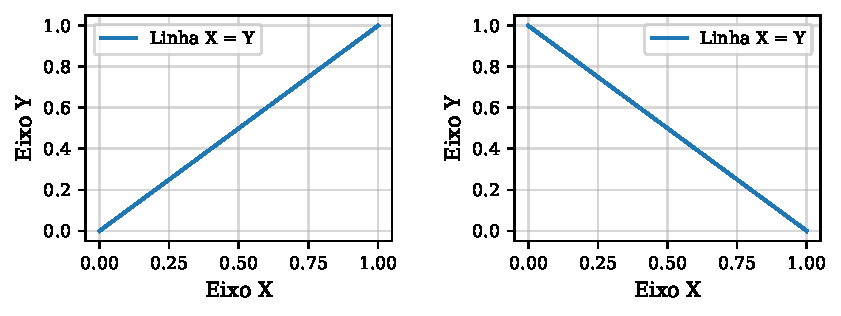
\includegraphics{exemplo_matplot_2.pdf}
          \caption{Exemplo de figura feita usando a função \ttt{set\_size}.}
          \label{fig:matplot_1}
        \end{figure}
        %
        \begin{figure}[h]
          \centering
          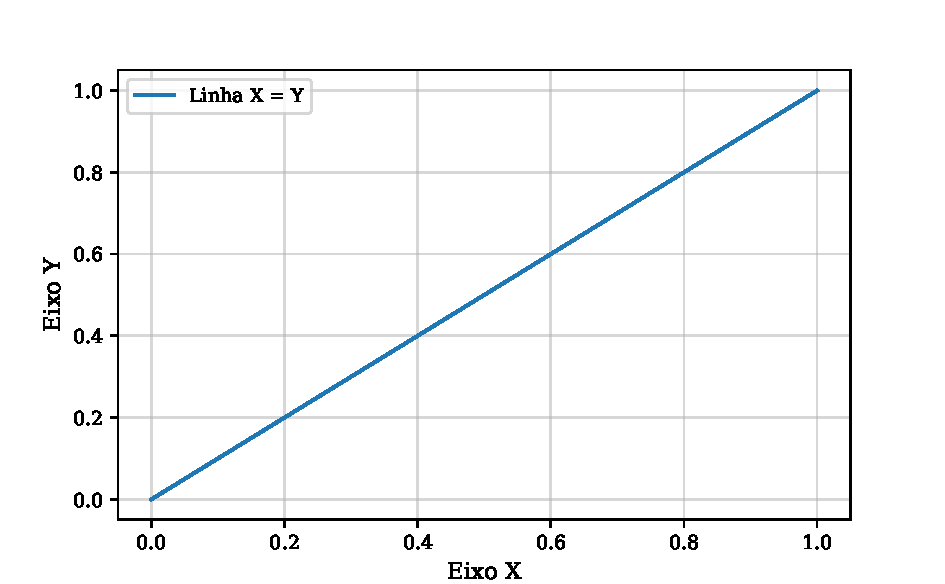
\includegraphics{exemplo_matplot.pdf}
          \caption{Exemplo de figura feita usando a função \ttt{set\_size}.}
          \label{fig:matplot_2}
        \end{figure}

        Note que nenhum caractere dentro da imagem tem tamanho menor do que os da legenda (que é um bom teste para saber se o tamanho das letras e números está bom) e como a imagem ocupa quase toda a largura do texto mesmo sem ser necessário usar a opção [width=\textbackslash linewidth].

      %     In this template, the citations are handled by the \ttt{natbib} package, with is defined by the commands in the ``Sections/6-bibliography.tex'' file. There, the list of used references are imported from the ``Sections/reference\_list.bib'' file.

  %     This package supports different types of citations, all of them explained here: \url{https://gking.harvard.edu/files/natnotes2.pdf}


  % The goal of this document is to provide an unofficial dissertation/thesis template for IAG/USP.

  % \section{General tips for when writing a dissertation/thesis}

  % When writing the text, you should be aware of the IAG/USP norms\footnote{\url{https://leginf.usp.br/?resolucao=resolucao-copgr-no-7882-de-25-de-novembro-de-2019}}. There are some obligatory chapters that should be in the text, the list is shown in ``XI – PROCEDIMENTOS PARA DEPÓSITO DA DISSERTAÇÃO/TESE''.

  % In order to make the deposit, you should have:
  % %
  % \begin{itemize}
  %   \item For PhD: a printed copy of the text, the forms containing the committee suggestion, a letter from the supervisor saying that you are fit for the defense, and proof of one published paper, where you are the first or second co-author, in a refereed international journal. You also need to make a deposit in Janus.
  %   \item For master's: 
  % \end{itemize}

  % IAG has a partnership with the IME's print shop. To print your dissertation/thesis with them you should send an email to \url{ccpastro iag.usp.br} with copy to \url{cida.coelho@iag.usp.br} asking for permission, with the PDF of the text attached. If approved, the text will be sent to the print shop and you will be notified when it is ready (within 1 or 2 days).

  % The forms for the committee and the supervisor manifestation can be found at IAG's website, in the ``Forms'' page: \url{https://www.iag.usp.br/pos-graduacao/formularios}. I recommend that you start thinking about the names that should be in your defense two weeks before making the deposit, and sending each member an email one week before, asking if they accept that their names be suggested.

  % \section{Features of this template}

  %   This template is based on the \ttt{WebLatex}\footnote{\url{https://github.com/sanjib-sen/WebLaTex}} template, created to replace Overleaf with Github, with some modifications. See the link for further details and the advantages of this approach.

  %   We also included the GitDoc extension, which automatically makes commit+push to a repository. To use it, you should enable the extension using \ttt{ctrl+shift+p} > ``GitDoc Enable''
  
  %   \subsection{Acronyms}
  %     The acronyms in this model are handled by the \ttt{acro} package, where you need to defined the acronyms beforehand, in the ``Sections/0.2-list\_of\_acronyms.tex'', using the format:

  %     \begin{lstlisting}[autogobble]
  %       \DeclareAcronym{acronym}{
  %         short = short name,
  %         long  = long name,
  %         cite  = citation %optional
  %       }
  %   \end{lstlisting}

  %   Using this package, the first reference to an acronym is written normally, with the reference if you defined the acronym with one, using the ``long'' name: \ac{splus}. Whenever you make another reference to this acronym, it will use the ``short'' name: \ac{splus}.
    
  %   You can also define acronyms using math-mode: \ac{photoz}. If you use the acronym only once, it will be printed using the long form only, without diplaying the short form, in this case, use can use the \ttt{\textbackslash ac\{acro\}} command followed by  \ttt{\textbackslash acuse\{acro\}}: \ac{specz}\acuse{specz}.

  %   There are some variations on how the acronyms can be printed, such as:
  %   \begin{itemize}
  %     \item Plural: \ttt{\textbackslash acp\{photoz\}} $\rightarrow$ \acp{photoz}
  %     \item Force long name: \ttt{\textbackslash acl\{des\}} $\rightarrow$ \acl{des}
  %     \item Force short name: \ttt{\textbackslash acs\{vhs\}} $\rightarrow$ \acs{vhs}
  %     \item Capital first letter: \ttt{\textbackslash Ac\{photoz\}} $\rightarrow$ \Ac{photoz}
  %   \end{itemize}

  %   \subsection{Citations}
  %     In this template, the citations are handled by the \ttt{natbib} package, with is defined by the commands in the ``Sections/6-bibliography.tex'' file. There, the list of used references are imported from the ``Sections/reference\_list.bib'' file.

  %     This package supports different types of citations, all of them explained here: \url{https://gking.harvard.edu/files/natnotes2.pdf}

  %   \subsection{Examples of tables, figures, listings...}

  %   \subsection{Making figures with \ttt{Matplotlib}}